\documentclass[tikz,border=12pt]{standalone}
% Shared visual language for standalone EMT block diagrams.
\usepackage{amsmath}
\usetikzlibrary{arrows.meta,backgrounds,calc,fit,positioning}

\tikzset{
    emt diagram/.style = {>={Stealth[length=2.4mm]}},
    line/.style        = {semithick, rounded corners=6pt},
    block/.style       = {draw, semithick, fill=white,
                          minimum height=1cm, minimum width=2.3cm},
    hblock/.style      = {block, minimum width=2.24cm, minimum height=1.3cm},
    vblock/.style      = {block, minimum width=1.3cm, minimum height=2.24cm},
    sum/.style         = {draw, semithick, fill=white, circle,
                          inner sep=2.6pt},
    signal/.style      = {circle, fill, inner sep=1.4pt,
                          label distance=3pt},
    sig/.style         = {font=\small},
    pm/.style          = {font=\scriptsize},
    wire jump/.style   = {line,
                          preaction={draw=white, line width=3pt,
                                     line cap=round}},
    enclosure/.style   = {draw, dashed, semithick, rounded corners=4pt},
    operator enclosure/.style = {enclosure, inner xsep=7mm, inner ysep=6mm}
}


\begin{document}
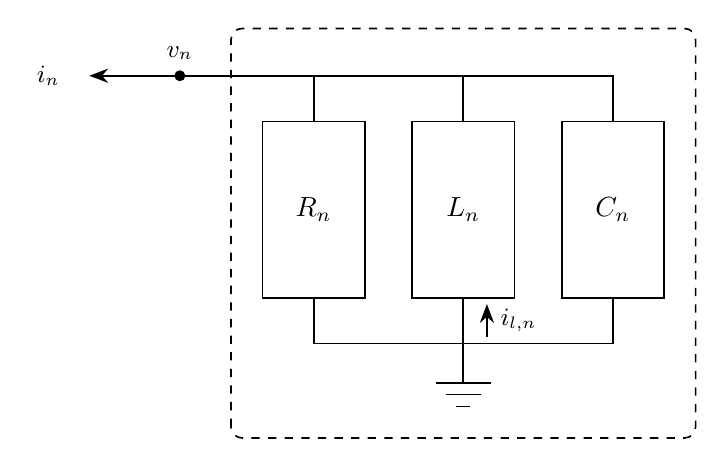
\begin{tikzpicture}[emt diagram]

% ================= Parallel branches =================
\node[vblock] (R) at (-1.9, -0.1) {$R_n$};
\node[vblock] (L) at (0, -0.1) {$L_n$};
\node[vblock] (C) at (1.9, -0.1) {$C_n$};
\coordinate (terminal) at (0, 1.6);
\coordinate (return) at (0, -1.8);
\draw[semithick] (R.north) |- (terminal) -| (C.north);
\draw[semithick] (terminal) -- (L.north);
\draw[semithick] (R.south) |- (return) -| (C.south);
\draw[semithick] (L.south) -- (return);

% ================= Inductor current =================
\draw[->, semithick] (0.3, -1.72) -- (0.3, -1.30);
\node[sig, anchor=west] at (0.35, -1.51) {$i_{l,n}$};

% ================= Terminal voltage and current =================
\node[signal, label={[sig]above:$v_n$}] (vport) at (-3.6, 1.6) {};
\draw[->, line] (-1.9, 1.6) -- (-4.75, 1.6);
\node[sig, anchor=east] at (-5.0, 1.6) {$i_n$};

% ================= Ground reference =================
\draw[semithick] (return) -- (0, -2.3);
\draw[semithick] (-0.35, -2.30) -- (0.35, -2.30);
\draw[semithick] (-0.22, -2.45) -- (0.22, -2.45);
\draw[semithick] (-0.09, -2.60) -- (0.09, -2.60);

% ================= Model enclosure =================
\draw[enclosure] (-2.95, -3.0) rectangle (2.95, 2.2);

\end{tikzpicture}
\end{document}
